% this file is called up by the header file
% content in this file will be fed into the main document
% ----------------------- paths to graphics ------------------------
\graphicspath{{figures/}}

% ----------------------- contents start here ------------------------

\chapter{Model}\label{chap:model}

\section{Channel Capacity, Noise and Signal Power}
In order to estimate the radio propagation losses in a given environment, 
a loss model has to be established. Given the loss model, the available 
transmission bandwith can be inferred with the Shannon-Hatley theorem \cite{hartley1928transmission} as followed: 

\begin{equation} \label{eq:capacity}
    C = B \log_2(1 + \frac{S}{N})
\end{equation}

where $C$ is the channel capacity (or bitrate), $B$ the bandwidth of the 
communication channel, $S$ the received signal power and $N$ the signal noise. 
Signal power over signal noise yield a fractionless unit, commonly called the 
signal to noise ratio (SNR). The SNR is given by the fraction $\frac{S}{N}$ for 
powers in Watts or by following subtraction $SNR = P_R - P_N$ if powers are 
given in decibels.\\
For a given channel model the bandwidth $B$ is known, leaving the $SNR$ to be 
determined. While the signal power $S$ is a more complex result of the recieved 
signal power minus transmission losses, the noise power $N$ is dominated by 
thermal noise in the receiving antenna and can be model by John-Nyquist noise. 
John-Nyquist noise models the thermal agitation of charge carriers in an electric
conductor \cite{nyquist1928thermal}, the antenna, and is given by: 
\begin{equation}
    P = k_B T \Delta f
\end{equation}
where $k_B$ is the Boltzmann constant, $T$ the temperature of the receiver in 
Kelvin and $\Delta f$ the bandwidth of the channel. Changes in temperature yield
negligable effect on the noise floor for common environmental temperature of $0$ 
to $30$ degress Celsisus. One can thus simplify the formula for a temperature
of $20$ degress Celsisus and express the power in units of $dBm$ (as will all 
upcoming formulas) to yield: 
\begin{equation} \label{eq:noise}
    P_N = 10 \log_{10}(k_B T * 1000) + 10 \log_{10}(\Delta f) = 174 + 10 \log_{10}(\Delta f)
\end{equation}
The noise power is thus primarily affected  on the channel bandwidth $\Delta f$. \\
The received signal power $P_R$ is modeled, for any given receiver-transmitter pair
of radio antennas, by the Friis transmission equation \cite{friis1946note}: 
\begin{equation} \label{eq:friis}
    P_R = P_T + G_T + G_R - 20 \log_{10} (\frac{4 \pi d}{\lambda})
\end{equation}
where $P_T$ is the transmission power in decibels at the transmitting antenna, 
$G_T$ and $G_R$ the transmitting and receiving antenna gains respectively. The 
last term gives the free-space path loss that the signal undergoes, given receiver
and transmitter and in the far field of each other ($d >> \lambda$), where $d$ 
gives the transmitter-receiver distance and $\lambda$ the carrier wavelength. 
For a 5 GHz signal, the wavelength equals $6$ cm. Thus the far field assumption holds
for the given case, as transmitter-receiver distances $d$ of less then $1$ m are
not of interest. \\

\section{Free-Space Path Loss}
The free-space path loss ($FSPL$) term of the Friis transmission equation (last term,\cite{sklar2001digital}) 
yields only the path loss due to the geometric spread of the tranmission signal over distance. To include
further environmental scenarios, such as non line of sight (NLOS) cases, the FSPL 
is replaced with the path loss ($PL$) given by the log normal shadowing (or 
large-scale path loss) model (\cite{seidel1991path}), as:
\begin{equation} \label{eq:pl-log}
    PL_L = FSPL(f, 1m) + 10 n \log_{10}(d) + \chi_{\sigma}
\end{equation}
The path loss is given by the $FSPL$ at a receiver-transmitter distance of $1$ m and 
extended by terms around the path loss exponent $n$ (or PLE) and the
fading deviation $\chi_{\sigma}$. One may note that a PLE $n$ of 2 would yield
the same as the FSPL at distance $d$ plus the deviation term $\chi_{\sigma}$. 
$PLE$ and $\chi_{\sigma}$ are found as results from experimental measurements. 
Figure \ref{fig:PLE} shows measurements under different environmental conditions
and the marks the according trend lines for the respective path loss exponents $n$. 
Values for $n$ and $\chi_{\sigma}$ are found in table \ref{tab:ple} for urban and rural environemtns
and line of sight and non line of sight scenarios. 

\begin{figure}[htb]
\begin{center}
    \begin{tabular}{ c | c | c }
        Environment & Path Loss Exponent & Fading Deviation [dB] \\
        \hline
        \hline
        Urban LOS & 2.0 & 4.0 \\
        \hline
        Urban NLOS & 3.2 & 7.0 \\
        \hline
        Rural LOS & 2.2 & 4.0 \\
        \hline
        Rural NLOS & 2.8 & 8.0 \\
        \hline
    \end{tabular}
    \caption{Table of common path loss exponents and fading deviation values for given LOS and NLOS environments. 
    Updated values taken from \cite{sun2017novel}.}
    \label{tab:ple}
\end{center}
\end{figure}

\begin{figure}[htb]
    \begin{center}
        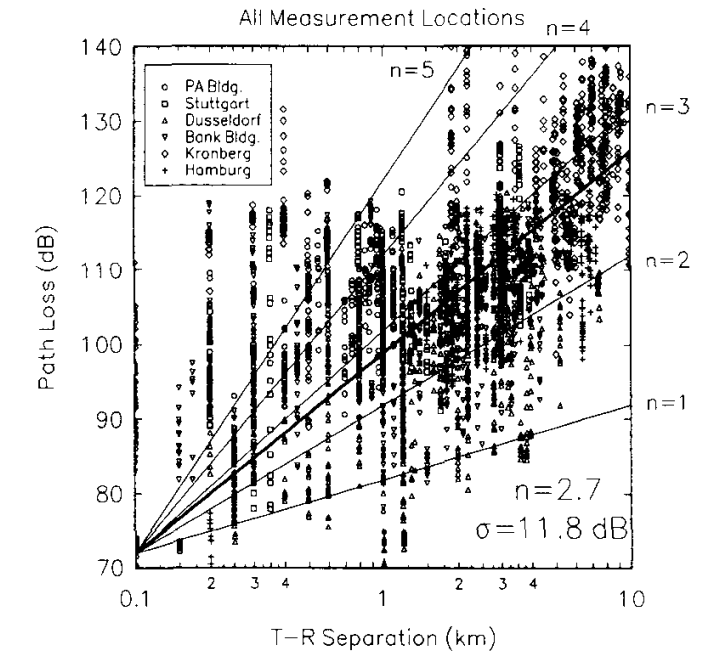
\includegraphics[width=0.8\textwidth]{smba_ple}
        \caption{Experimentally determined path loss vs log transmitter-receiver distance for various environments.
        Trend lines indicate the path loss exponent for given scenarios \cite{seidel1991path}.}
        \label{fig:ple}
    \end{center}
\end{figure}


\section{Specific path losses}
\subsection{Foliage}
Signal attenuation due to foliage can be described by Weissberger's model \cite{weissberger1982initial}. Based 
on experimental data, a formula is given for foliage depth $d_f$ of up to 400m, 
for a given channel of carrier frequency $f$ as followed: 
\begin{equation} \label{eq:pl-foliage}
    PL_F = 
    \begin{cases}
        1.33 f^{0.284} d_f^{0.588} & \text{if $14 < d \leq 400$} \\
        0.45 f^{0.284} d_f         & \text{if $0  < d \leq 14$}
    \end{cases}
\end{equation}
Wiessberger's model is best for dense, dry tree foliage and only suitable for carrier
frequencies between $230$ MHz and $95$ GHz. The frequency criteria is fullfilled in the 
channel models followingly investigated and the model sufficiently applicable to middle 
european vegetation. 

\subsection{Rainfall}
A model for path loss due to rainfall is given by the International Telecommunications Union
(ITU) in recommondation ITU-R P.838-3 \cite{itu838-3}. The recommondation (based on \cite{liebe1993propagation}) 
specifies the specific 
attenuation $\gamma_R$ in dB/km (transmitter-receiver distance) for a given rainfall rate $R$ 
in mm/h as followed: 
\begin{equation} \label{eq:itu-atten}
    \gamma_R = k R^{\alpha}
\end{equation}
whereby the coefficients $k$ and $\alpha$ are given for linear or circular polarizations by: 
\begin{equation}
    k = [ k_H + k_V + ( k_H - k_V ) \cos^2 \theta \cos 2 \tau ] / 2 \\
\end{equation}
\begin{equation}
    \alpha = [ k_H \alpha_H + k_V \alpha_V + ( k_H \alpha_H - k_V \alpha_V) \cos^2 \theta \cos 2 \tau ] / 2 k
\end{equation}
The recommondation provides lookup tables for the horizontal and vertical components of $k$ and $\alpha$ 
for carrier frequencies $f$ between 1 and 1000 GHz. For simplicity, only the values at 28 GHz
are used in the following model, which avoids implementing a lookup table for the given coefficients.
To get the path loss in dB, equation \ref{eq:itu-atten} must be multiplied by the distance $d$ as followed: 
\begin{equation} \label{itu-pl}
    PL_R = k R^{\alpha} d / 1000
\end{equation}

As rainfall attentuation increases for carrier freuencies $f$ below 100 GHz (as seen in figure \ref{fig:itu_rainfall}, 
the choosen frequency provides us with an upper limit for the targeted 5G frequencies of 2 to 28 GHz.
One may note, that for even for heavy rainfall, as assumed in figure \ref{fig:itu_rainfall}, the path loss
due to rainfall is below 1dB and thus negligably small.

\begin{figure}[htb]
    \begin{center}
        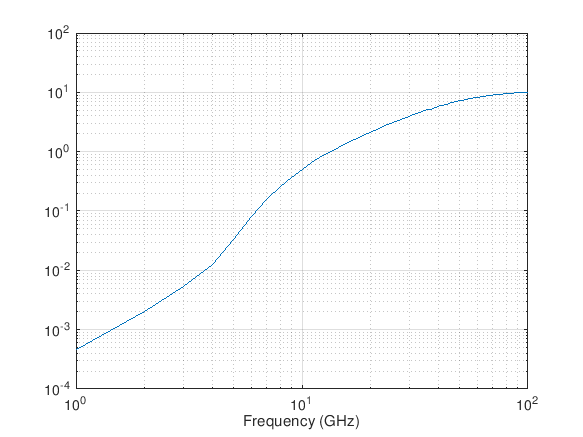
\includegraphics[width=0.9\textwidth]{smba_itu_rainfall}
        \caption{Plot of path loss (attenuation) due to heavy rainfall (20mm/h) for carrier frequencies between 1 and 100 GHz, 
        given a transmitter receiver distance of 1000m. (MathWorks Matlab Phased Array System Toolbox)}
        \label{fig:itu_rainfall}
    \end{center}
\end{figure}

\section{Channel Model}
Given all models for signal attenuation above, a final path loss can be constructed (\cite{tse2005fundamentals}) from equations 
\ref{eq:pl-log}, \ref{eq:pl-foliage} and \ref{eq:itu-atten} as: 
\begin{equation} \label{eq:pl-sum}
    \begin{split}
        PL & = PL_L + PL_F + PL_R \\
             & = 20 \log_{10} (\frac{4 \pi f}{c}) + 10 n \log_{10}(d) + \chi_{\sigma} \\
             & \quad + 1.33 f^{0.284} d_f^{0.588} \\
             & \quad + k R^{\alpha} d / 1000
    \end{split}
\end{equation}
given $14 < d_f \leq 400$ for Weissenberg's model case. The accompanying python implementation of the channel 
model does account for both cases accordingly. 

The final channel capacity can thus be obtained by substituting the path loss equation \ref{eq:pl-sum} into 
Friis transmission equation \ref{eq:friis}: 
\begin{equation} \label{eq:friis-final}
    P_R = P_T + G_T + G_R - PL
\end{equation}

Shannon-Nyquist (\ref{eq:capacity}) then yields the final capacity in bits/second through Friis (\ref{eq:friis-final}) 
and the Nyquist noise (\ref{eq:noise}) as: 
\begin{equation} \label{eq:capacity}
    C = B \log_2(1 + SNR) = B \log_2(1 + 10^{( (P_R-P_N) / 10 )} )
\end{equation}


Simulation results for various scenarios with channel model given above are presented in the next chapter.

